\section{Opis i treść kodu PythonPIC}
Cały kod programu w celu reprodukowalności wyników tworzony był i jest
dostępny na platformie GitHub\cite{github-repo}.

Program ma obiektową strukturę zewnętrzną, którą w celu łatwości
zrozumienia jego działania nakrywa wewnętrzną warstwę składającą się
głównie z n-wymiarowych tablic \code{numpy.ndarray} oraz zwektoryzowanych
operacji na nich.

Część symulacyjna kodu składa się z kilku prostych koncepcyjnie elementów:

\subsection{Grid - siatka Eulera}
Klasa reprezentująca dyskretną siatkę Eulera, na której dokonywane są
obliczenia dotyczące pól elektromagnetycznych oraz gęstości ładunku i
prądu.  Zawiera:
\begin{itemize}
    \item $x_i$ - tablicę położeń lewych krawędzi komórek siatki
    \item $N_G$ - liczbę komórek siatki
    \item $T$ - sumaryczny czas trwania symulacji
    \item $\Delta x$ - krok przestrzenny siatki - $N_G \Delta x$ daje
        długość obszaru symulacji
    \item $\rho_i$ - tablicę gęstości ładunku na siatce.
    \item $\vec{j}_{i,j}$ - tablicę gęstości prądu na siatce.
    \item $E_{i,j}$ - tablicę pola elektrycznego na siatce.
    \item $B_{i,j}$ - tablicę pola magnetycznego na siatce.
    \item $c$, $\varepsilon_0$ - stałe fizyczne - prędkość światła oraz
        przenikalność elektryczną próżni.
    \item $\Delta t$ - krok czasowy symulacji, obliczony jako $\Delta t =
        \Delta x / c$.
    \item $N_T$ - liczbę iteracji czasowych symulacji.
    \item \code{BC} - \emph{Boundary Condition}, obiekt zawierajacy informacje dotyczace
        warunku brzegowego zadanego na pole elektryczne i magnetyczne. W przypadku symulacji
        laserowej jest to subklasa Laser zawierajaca informacje o dlugosci fali, ksztalcie obwiedni
        i polaryzacji impulsu. W kazdej iteracji \code{BC} poprzez metode
        \code{apply} aktualizuje wartosci na lewym brzegu siatki obliczeniowej.
        %wartość warunku brzegowego dotyczącego natężenia fali
        %elektromagnetycznej (laserowej) wchodzącej do pola symulacji z
        %lewej strony.
\end{itemize}

Istotne metody klasy \code{Grid}, o których należy wspomnieć, to:
\begin{itemize}
     \item \code{apply\_bc} - aktualizuje krańcowe wartości tablic $E$, $B$
         w oparciu o podany warunek brzegowy.
     \item gather\_current \todo[inline]{finish these}
     \item gather\_charge
     \item solve
     \item field\_solve
     \item electric\_field\_function, magnetic
     \item save\_to\_h5py
\end{itemize}

\subsection{Species - cząstki}
Klasa reprezentująca pewną grupę makrocząstek o wspólnych cechach, takich
jak ładunek bądź masa.  Przykładowo, w symulacji oddziaływania lasera z
tarczą wodorową jedną grupą są protony, zaś drugą - elektrony.  Do
zainicjalizowania wymaga instancji \code{Grid}, z której pobiera informacje
takie jak stałe fizyczne $c$, $\varepsilon_0$, liczbę iteracji czasowych
$N_T$ i czas trwania iteracji $\Delta t$.

Zawiera skalary:
\begin{itemize}
    \item $N$ - liczba makrocząstek
    \item $q$ - ładunek cząstki
    \item $m$ - masa cząstki
    \item \code{scaling} - liczba rzeczywistych cząstek, jakie reprezentuje
        sobą makrocząstka. Jej sumaryczny ładunek wynosi $q *
        $\code{scaling}, masa $m * $\code{scaling}.
    \item \code{N\_alive} - liczba cząstek obecnie aktywnych w symulacji.
        Zmniejsza się w miarę usuwania cząstek przez warunki brzegowe.
\end{itemize}

Poza skalarami zawiera tablice rozmiaru $N$:
\begin{itemize}
    \item jednowymiarowych położeń makrocząstek $x^n$, zapisywanych w
        iteracjach $n, n+1, n+2$\ldots
    \item trójwymiarowych prędkości makrocząstek $\vec{v}^{n+\frac{1}{2}}$,
        zapisywanych w iteracjach $n+\frac{1}{2}, n+{3}{2}, n+{5}{2}$\ldots
    \item stanu makrocząstek (flagi boolowskie oznaczające cząstki aktywne
        bądź usunięte z obszaru symulacji)
\end{itemize}

Poza tym, zawiera też informacje dotyczące zbierania danych diagnostycznych
dla cząstek, niepotrzebnych bezpośrednio w czasie symulacji:
\begin{itemize}
    \item \code{name} - słowny identyfikator grupy cząstek, dla potrzeb legend wykresów
    \item $N_T$ - liczbę iteracji czasowych w symulacji
    \item $N_T^s$ - zmniejszoną liczbę iteracji, w których następuje pełne
        zapisanie położeń i prędkości cząstek.  Dane te są wykorzystywane
        do tworzenia diagramów fazowych cząstek.
    \item odpowiadające poprzednio wymienionym tablice rozmiaru $(N_T^s,
        N)$, $(N_T^s, N, 3)$.  \item jedną tablicę rozmiaru $(N_T, N_G)$
        dotyczącą zebranych podczas
        depozycji ładunku informacji diagnostycznych o przestrzennej
        gęstości cząstek.
    \item trzy tablice rozmiaru $(N_T)$ dotyczącą średnich prędkości,
        średnich kwadratów prędkości i odchyleń standardowych prędkości.
\end{itemize}

Jeżeli liczba makrocząstek lub iteracji przekracza pewną stałą, dane zapisywane są jedynie dla co $n$-tej cząstki,
gdzie $n$ jest najniższą liczbą całkowitą która pozwala na zmniejszenie tablic poniżej tej stałej.

Warto wspomnieć o metodach klasy \code{Species}:
\begin{itemize}
    \item push \todo[inline]{fill these}
\end{itemize}

\subsection{Simulation}
Klasa zbierająca w całość Grid oraz dowolną liczbę Species zawartych w
symulacji, jak również pozwalająca w prosty sposób na wykonywanie iteracji
algorytmu i analizy danych. Jest tworzona tak przy uruchamianiu symulacji,
jak i przy wczytywaniu danych z plików \code{.hdf5}.

\begin{itemize}
    \item $\Delta t$ - krok czasowy
    \item $N_T$ - liczba iteracji w symulacji
    \item \code{Grid} - obiekt siatki
    \item \code{list\_species} - lista grup makrocząstek w symulacji
\end{itemize}
\todo[inline]{metody simulation}

Przygotowanie warunków początkowych do danej symulacji polega na utworzeniu
nowej klasy dziedziczącej po \code{Simulation}, która przygotowuje siatkę,
cząstki i warunki brzegowe zgodnie z założeniami eksperymentu i wywołuje
konstruktor \code{Simulation}.  Należy również przeciążyć metodę
\code{grid\_species\_init}, która przygotowuje warunki początkowe. Domyślna
wersja tej metody wykonuje pierwszą, początkową iterację równań ruchu,
która pozwala na zachowanie symplektyczności integratora równań ruchu,
\todo[inline]{stylistyka?} co pomaga zachować energię cząstek w symulacji.
W tym momencie jest tez tworzony plik \code{.hdf5}, do ktorego zapisywane sa
dane gromadzone w czasie symulacji.

Aby uruchomić symulację, należy wywołać jedną z metod:
\begin{itemize}
     \item \code{run} - podstawowy cykl obliczeń, używany do pomiarów
         wydajności programu
     \item \code{test\_run} - obliczenia oraz obróbka danych na potrzeby
         analizy, głównie stosowana w testach
     \item \code{lazy\_run} - \code{test\_run} z zapisem do pliku oraz
         wczytaniem z pliku \emph{.hdf5}, jeżeli początkowe warunki oraz
         wersja kodu zgadzają się. W przeciwnym razie symulacja zostaje
         uruchomiona na nowo.
\end{itemize}

\subsection{Pliki pomocnicze}
Poza powyższymi program jest podzielony na pliki z implementacjami algorytmow numerycznych,
co pozwala na zwiekszenie niezaleznosci testow oraz zwieksza modularnosc kodu.
\begin{itemize}
    \item BoundaryCondition
    \item FieldSolver
    \item particle\_push
    \item field\_interpolation

    \item algorithms\_grid - zawiera algorytmy dotyczące rozwiązywania
        równań Maxwella na dyskretnej siatce

    \item algorithms\_interpolation - zawiera algorytmy interpolujące pola
        z cząstek na siatkę i odwrotnie
    \item algorithms\_pusher - zawiera algorytmy integrujące numerycznie
        równania ruchu cząstek
    \item animation - tworzy animacje dla celów analizy danych
    \item static\_plots - tworzy statyczne wykresy dla celów analizy danych
    \item plotting - zawiera ustawienia dotyczące analizy danych
        \todo[inline]{czy to można przenieść do simulation czy gdzieś?}
\end{itemize}

Przygotowane konfiguracje istniejących symulacji są zawarte w plikach
\code{configs/run\_*}: \todo[inline]{przeformułować}
\begin{itemize}
    \item run\_coldplasma
    \item run\_twostream
    \item run\_wave
    \item run\_beam
    \item run\_laser
\end{itemize}

Algorytmiczne testy jednostkowe są zawarte w katalogu \code{tests}.

\subsection{Wykorzystane biblioteki Pythona}

Pomijamy tutaj bibliotekę standardową jako wbudowaną w sam język.

\subsubsection{Numpy}
\code{numpy}\cite{numpy} to biblioteka umożliwiająca wykonywanie złożonych obliczeń na
n-wymiarowych macierzach bądź tablicach, utworzona w celu umożlwiienia
zastąpienia operacjami wektorowymi iteracji po tablicach, powszechnie
stosowanych w metodach numerycznych i będących znanym słabym punktem
Pythona.

Pod zewnętrzną powłoką zawiera odwołania do znanych, wypróbowanych i
sprawdzonych w numeryce modułów \code{LAPACK}, \code{BLAS} napisanych w
szybkich, niskopoziomowych językach C oraz \code{FORTRAN}.  Jest to
\emph{de facto} standard większości obliczeń numerycznych w Pythonie.

Należy zauważyć, że operacje matematyczne w wersji \code{numpy} zawartej
w dystrybucji Anaconda są automatycznie
zrównoleglane tam, gdzie pozwala na to
niezależność obliczeń dzięki dołączonym bibliotekom Intel Math Kernel Library.\cite{intel-mkl} 

Numpy jest oprogramowaniem otwartym, udostępnianym na licencji BSD.


\subsubsection{scipy}
Kolejną podstawową biblioteką w numerycznym Pythonie jest \code{scipy},
biblioteka zawierająca wydajne gotowe implementacje wielu powszechnych algorytmów
numerycznych służących między innymi całkowaniu, optymalizacji funkcji rzeczywistych,
uczeniu maszynowemu, algebrze liniowej czy transformatom Fouriera.

\subsubsection{Numba}
\code{numba} to biblioteka służąca do kompilacji just-in-time wysokopoziomowego
kodu Pythona do kodu niskopoziomowego przy pierwszym uruchomieniu programu. W
wielu przypadkach pozwala na osiągnięcie kodem napisanym w czystym Pythonie
wydajności marginalnie niższej bądź nawet równej do analogicznego programu w C
bądź Fortranie. \cite{numba}

Jednocześnie należy zaznaczyć prostotę jej użycia. W wielu przypadkach wystarczy
dodać do funkcji dekorator \code{@numba.jit}:


\lstinputlisting[language=Python, numbers=left, caption=Przykład zastosowania kompilacji just-in-time z biblioteki Numba wykorzystujący metody pomiaru czasu środowiska Jupyter.]{listings/numba_example.py}

Istniejącym od niedawna kodem symulacyjnym implementującym tą metodę jest FBPIC\cite{fbpic}.


\subsubsection{HDF5}
HDF5 jest wysokowydajnym formatem plikow służącym przechowywaniu danych
liczbowych w drzewiastej, skompresowanej strukturze danych, razem z
równoległym, wielowątkowym zapisem tych danych.  W Pythonie implementuje go
biblioteka h5py\cite{h5py}.

W bieżącej pracy wykorzystuje się go do przechowywania danych liczbowych
dotyczących przebiegu symulacji, pozwalających na ich dalsze przetwarzanie
i analizę poprzez wizualizację.

\subsubsection{matplotlib}
Do wizualizacji danych z symulacji (oraz tworzenia schematów w sekcji
teoretycznej niniejszej pracy) użyto własnoręcznie napisanych skryptów w
uniwersalnej bibliotece graficznej \code{matplotlib}\cite{matplotlib}.
\code{matplotlib} zapewnia wsparcie zarówno dla grafik statycznych w różnych układach
współrzędnych (w tym 3D), jak również dla dynamicznie generowanych animacji
przedstawiających przebiegi czasowe symulacji.

\subsubsection{py.test}
Przy pracy nad kodem użyto frameworku testowego \code{py.test}~\cite{pytest}.
Tworzenie testów jest trywialne:

\lstinputlisting[language=Python, numbers=left, caption=Podstawowy przykład testu w pliku \code{func.py}]{listings/func.py}

Uruchamianie zaś:

\begin{lstlisting}[language=Bash]
    >>> pytest func.py
    === FAILURES ===
    ___failing ___

        def test_failing():
    >       assert f(4) == 13
    E       assert 12 == 13
    E        +  where 12 = f(4)

    func.py:10: AssertionError
    === 1 failed, 1 passed in 0.10 seconds ===
\end{lstlisting}

Należy zaznaczyć, że w numeryce, gdzie błędne działanie programu nie
objawia się zazwyczaj formalnym błędem, a jedynie błędnymi
wynikami, dobrze zautomatyzowane testy jednostkowe potrafią zaoszczędzić
bardzo dużo czasu na debugowaniu poprzez automatyzację uruchamiania
kolejnych partii kodu i lokalizację błędnie działających części algorytmu.
Dobrze napisane testy są praktycznie koniecznością w dzisiejszych czasach,
zaś każdy nowo powstały projekt numeryczno-symulacyjny powinien je
wykorzystywać, najlepiej do weryfikacji każdej części algorytmu z osobna.

Dobrym przykładem skutecznego testu jednostkowego jest porównanie energii kinetycznej
elektronu o znanej prędkości z wartością tablicową, zawarte jako test w pliku
\code{pythonpic/tests/test\_species.py}.

\code{py.test} jest oprogramowaniem otwartym, dostępnym na licencji MIT.

\subsubsection{Travis CI}
Nieocenionym narzędziem w pracy nad kodem był system ciągłej integracji
(\emph{continuous integration}) Travis CI \cite{travisci}
dostępny za
darmo dla projektów open-source. Travis pobiera aktualne wersje kodu przy
każdej aktualizacji wersji dostępnej na serwerze GitHub i uruchamia testy,
zwracając komunikat o ewentualnym niepowodzeniu i pozwalając na jednoczesne
uruchamianie bieżących, intensywnych symulacji przy jednoczesnym
weryfikowaniu w chmurze poprawności działania lżejszych, acz wciąż intensywnych
symulacji testowych i testów algorytmicznych.

\subsubsection{snakeviz}

W optymalizacji przydatny okazał się program \code{snakeviz}\cite{snakeviz} dostępny na
GitHubie i pozwalający na wizualizację wyników z profilowania
symulacji. Pozwala w wygodny sposób zbadać, które fragmenty kodu najbardziej
spowalniają symulację, które są najlepszymi kandydatami do optymalizacji, oraz
jak skuteczne (bądź nieskuteczne) okazują się próby polepszenia ich wydajności.
Działanie programu ilustruje rysunek~\ref{fig:snakeviz}.
\begin{figure}[h!]
  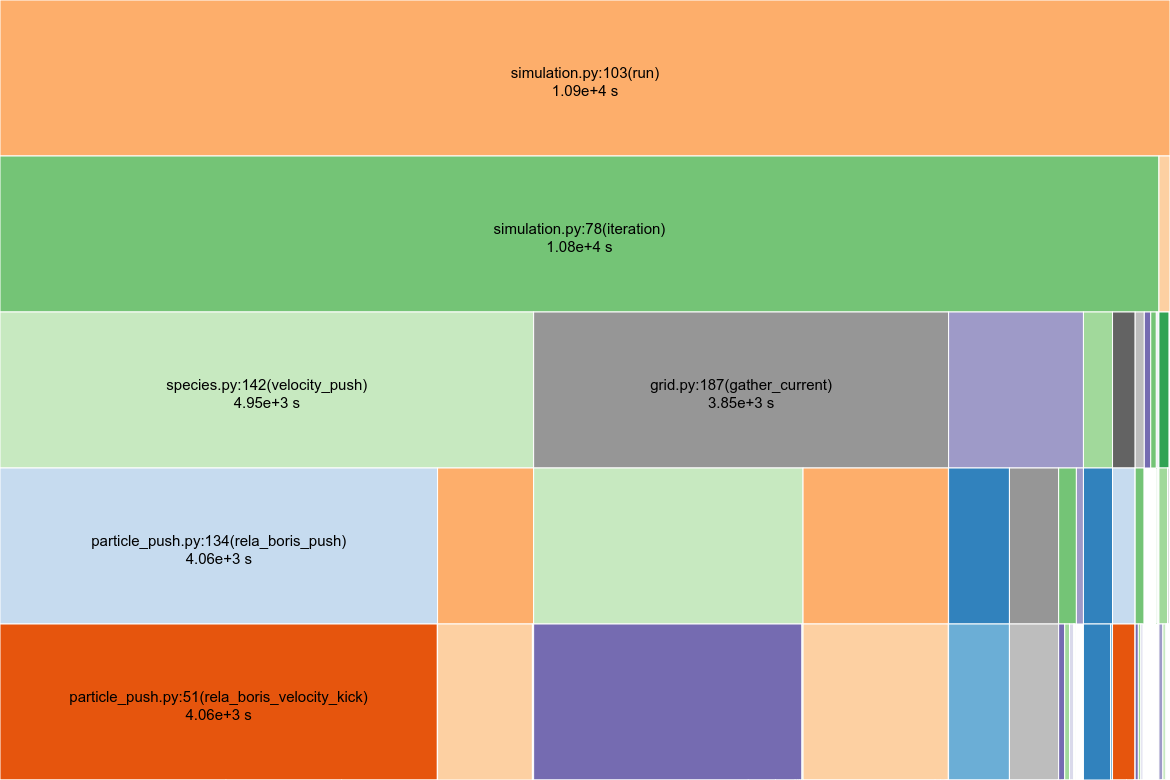
\includegraphics[width=\textwidth]{Images/snakeviz}
  \caption{Wizualizacja szybkości działania poszczególnych fragmentów kodu
    wygenerowana programem snakeviz.}
  \label{fig:snakeviz}
\end{figure}
